\section*{Velocity-Acceleration Plot}
\begin{frame}{Velocity-Acceleration Plot}
    The velocity-acceleration plot is a diagram
    with velocity on the $x$-axis
    and (longitudinal) acceleration on the $y$-axis.
    \begin{center}
        \begin{tikzpicture}
            \begin{axis}[axis lines=center, xmin=0, xmax=55, ymin=-3, ymax=3]
                \pgfplotsset{xlabel={$v_x$}, ylabel={$a_x$}}
            \end{axis}
        \end{tikzpicture}
    \end{center}
    This is known as a \textbf{state space} diagram.
\end{frame}

\begin{frame}
    Lets add some limits to the graph.
    We will begin by drawing a free-body diagram of a car.
    \begin{center}
        \begin{tikzpicture}
            \node (freebody) at (0,0) {%
                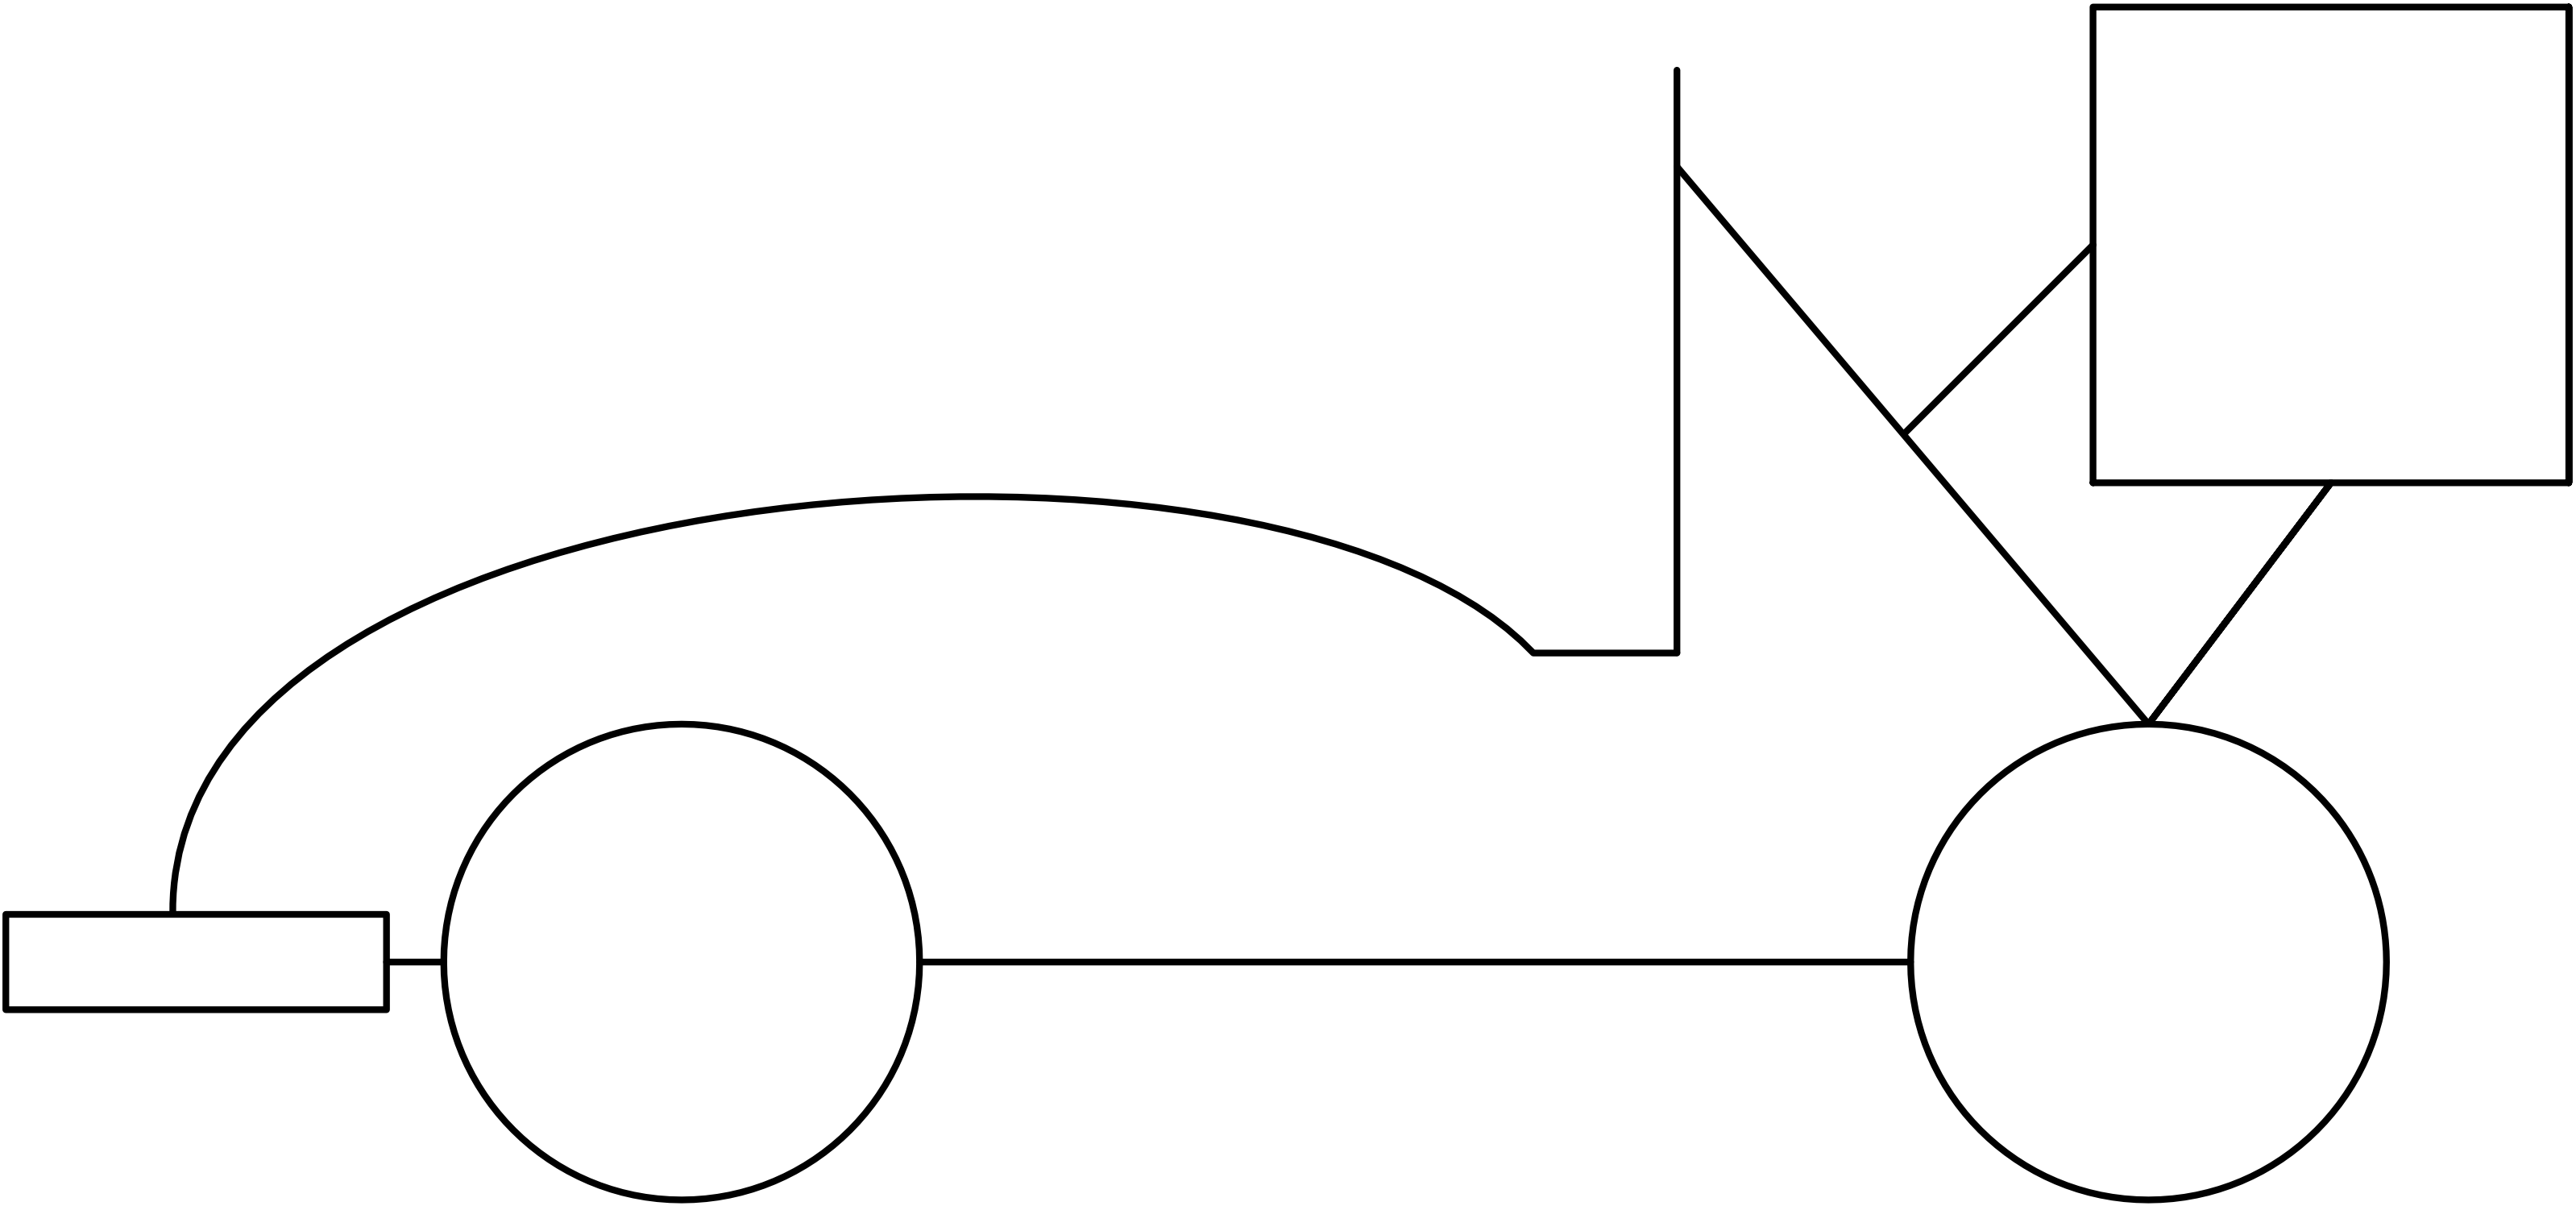
\includegraphics[width=0.8\textwidth]{../../res/Free Body Car.png}
            };
            \node[above] (CoG) at (0,0) {$CoG$};
            \node[above] (CoP) at (1,0) {$CoP$};
            \node (TyreF) at (-2.15,-2) {};
            \node (TyreR) at (3.05,-2) {};
            \draw[thick,main,-latex] (CoG) -- ++(0,-2) node[right] {$W$};
            \draw[thick,main,-latex] (CoP) -- ++(0,-2) node[right] {$F_L$};
            \draw[thick,main,-latex] (1,0) -- ++(2,0);
            \node[above] at (2,0) {$F_D$};
            \draw[thick,main,latex-] (3.2,-2.1) -- ++(2,0) node[below] {$F_T$};
            \draw[thick,main,latex-] (TyreF) -- ++(0,-1) node[right] {$R_F$};
            \draw[thick,main,latex-] (TyreR) -- ++(0,-1) node[right] {$R_R$};
        \end{tikzpicture}
    \end{center}
\end{frame}

\begin{frame}
    Consider the forces acting horizontally (the $x$-direction):
    \begin{gather*}
        F_T = \frac{P}{v} \\
        F_D = \frac{1}{2} \rho C_D A v^2
    \end{gather*}
    The acceleration of the vehicle is the sum of these forces:
    \begin{align*}
        a_x &= \frac{1}{m} \sum F_x \\
        &= \frac{1}{m} \left(\frac{P}{v} - \frac{1}{2} \rho C_D A v^2\right) \\
        &= \frac{P}{mv} - \frac{\rho C_D A v^2}{2m}
    \end{align*}
    This is known as the \textbf{power limit} of the vehicle.
\end{frame}

\begin{frame}
    Acceleration is also limited by the grip available from the tyres. \\
    First, we calculate the normal force on the tyres:
    $$N = W + F_L = mg + \frac{1}{2} \rho C_L A v^2$$
    For a tyre with a constant coefficient of friction $\mu$, the maximum grip available is:
    $$F_f = \mu N = \mu \left(mg + \frac{1}{2} \rho C_L A v^2\right)$$
    Therefore, the \textbf{traction-limited} acceleration is:
    $$a_x = \frac{F_f - F_D}{m}
    = \frac{\mu}{m} \left(mg + \frac{1}{2} \rho C_L A v^2\right) - \frac{\rho C_D A v^2}{2m}
    = \mu g + \frac{\rho A(\mu C_L - C_D)}{2m} v^2$$
    Real tyres are \textbf{load sensitive},
    meaning that $\mu$ decreases as $N$ increases.
    This means that adding more downforce has diminishing returns.
\end{frame}

\begin{frame}
    Finally, the top speed of the car is limited
    by the top speed of the motor, $\omega_\text{max}$,
    which can be found on the motor's datasheet
    (try searching for \textit{`Emrax 228 datasheet'}). \\~\\
    This is divided by the final drive ratio
    to find the rotational velocity of the wheels,
    and multiplied by the tyre radius to find the
    \textbf{velocity limit} of the car.
    $$v_\text{max} = \frac{\omega_\text{max} R_0}{\text{FDR}}$$
\end{frame}

\begin{frame}
    Lets plot these three lines on the velocity-acceleration diagram:
    \begin{figure}
        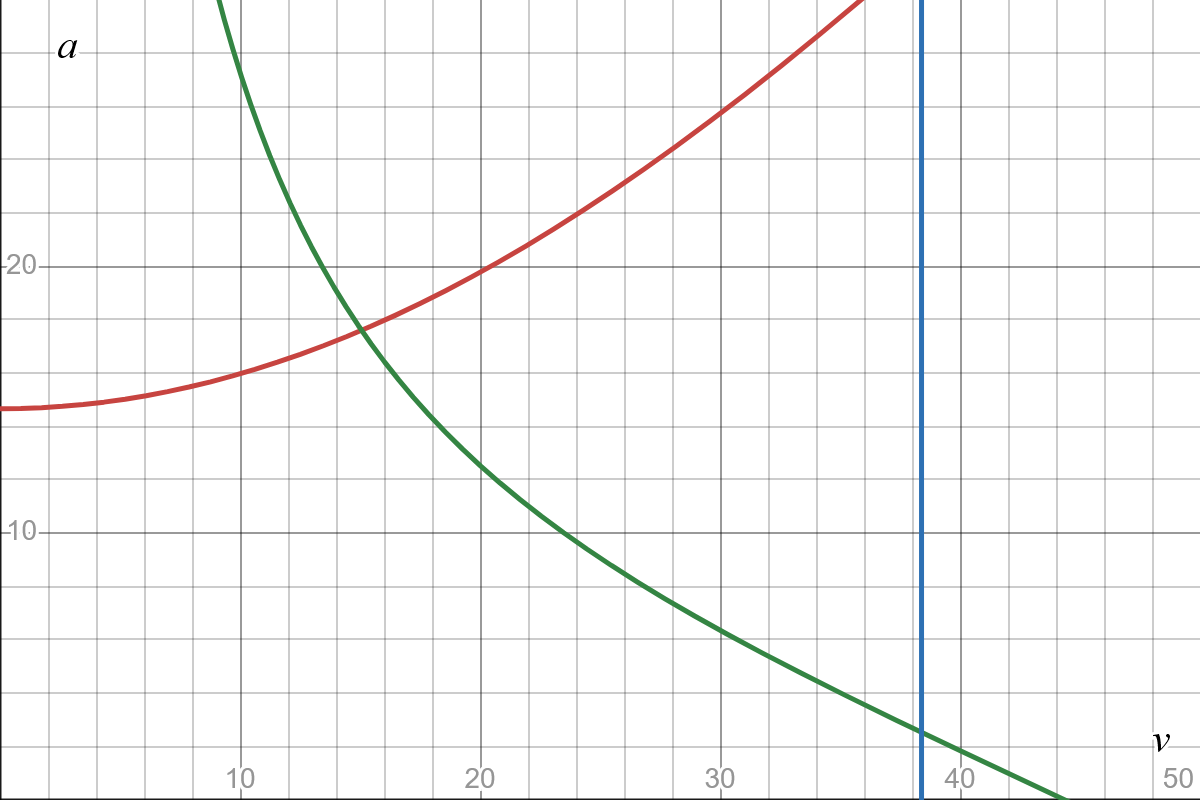
\includegraphics[width=\textwidth]{res/velocity-acceleration graph.png}
    \end{figure}
\end{frame}

\begin{frame}
    What does this graph tell us?
    \begin{itemize}
        \item At low velocities, acceleration is limited by traction
        \item The traction limit is governed by downforce and tyre grip
        \item At high velocities, acceleration is limited by power
        \item The power limit is governed by drag and motor power
    \end{itemize}
    You can open the graph in Desmos
    \href{https://www.desmos.com/calculator/vfyipxhjrg}{(\textit{link})}
    and move the vehicle parameter sliders
    to see how they affect the limits.
    \begin{block}{Try it yourself}
        This graph shows forward acceleration.
        What would the graph for braking look like?
    \end{block}
\end{frame}